%================================================================
% SLO
%----------------------------------------------------------------
% datoteka: 	thesis_template.tex
%
% opis: 		predloga za pisanje diplomskega dela v formatu LaTeX na
% 				Univerza v Ljubljani, Fakulteti za računalništvo in informatiko
%
% pripravili: 	Matej Kristan, Zoran Bosnić, Andrej Čopar,
%			  	po začetni predlogi Gašperja Fijavža
%
% popravil: 	Domen Rački, Jaka Cikač, Matej Kristan
%
% verzija: 		30. september 2016 (dodan razširjeni povzetek)
%================================================================


%================================================================
% SLO: definiraj strukturo dokumenta
% ENG: define file structure
%================================================================
\documentclass[a4paper, 12pt]{book}
 

%================================================================
% SLO: Odkomentiraj "\SLOtrue " za izbiro slovenskega jezika
% ENG: Uncomment "\SLOfalse" to chose English languagge
%================================================================
\newif\ifSLO
\newif\ifTRACKEXIST
\newif\ifTRACKCS
\newif\ifPROGRAMMM
\newif\ifPROGRAMEMAI


% ---------------------------------------------------------------------------------------
% IMPORTANT: Adjust the thesis language, your study program and track within this block
% ---------------------------------------------------------------------------------------
% ** switch language ** %
\SLOtrue % Enables Slovenian language
%\SLOfalse  % Enables English language

% ** Switch programs: ** %

% ** Uncomment if Program: Computer Science, Track: Computer Science **%
\TRACKCStrue
\TRACKEXISTtrue

% ** Uncomment if Program: Computer Science, Track: Data Science **%
%\TRACKCSfalse
%\TRACKEXISTtrue

% ** Uncomment if Program: Multimedia **%
%\PROGRAMMMtrue 
%\TRACKEXISTfalse 

% ** Uncomment if Program: EMAI **%
%\PROGRAMEMAItrue
%\SLOfalse 

% -------------------------------------------------------------------------------------------
% End of language, program and track adjustment
% -------------------------------------------------------------------------------------------


%================================================================
% SLO: vključi oblikovanje in pakete
% ENG: include design and packages
%================================================================
\input{style/thesis_style}

%----------------------------------------------------------------
% SLO: paketi in slogi za diagrame
% ENG: packages and styles for diagrams
%----------------------------------------------------------------
\usepackage{tikz}
\usetikzlibrary{arrows.meta,shapes.geometric,fit,backgrounds}
\tikzset{
	diagram/.style={font=\footnotesize, >={Stealth[length=1.8mm,width=1.5mm]}},
	blok/.style={draw, rounded corners=1.5pt, fill=white, align=center, inner sep=3pt},
	zbirka/.style={draw, cylinder, shape border rotate=90, aspect=0.09, fill=gray!12,
	               align=center, inner sep=3pt},
	tok/.style={->, semithick},
	oznaka/.style={font=\scriptsize, inner sep=1.5pt},
	okvir/.style={draw=gray!65, dashed, rounded corners=3pt, fill=gray!4,
	              inner xsep=3mm, inner ysep=3.5mm},
	naslov/.style={font=\scriptsize\bfseries, fill=white, inner xsep=2pt, inner ysep=1pt},
}

%----------------------------------------------------------------
% |||||||||||||||||||||| USTREZNO POPRAVI |||||||||||||||||||||||
% |||||||||||||||||||||| EDIT ACCORDINGLY |||||||||||||||||||||||
%----------------------------------------------------------------
\newcommand{\ttitle}{Agentni sistem za priporočanje izbire jezikovnega modela}
\newcommand{\ttitleEn}{Agent-based system for recommending the choice of a language model}
\newcommand{\tsubject}{\ttitle}
\newcommand{\tsubjectEn}{\ttitleEn}
\newcommand{\tauthor}{Peter Klepec}
\newcommand{\temail}{peter.klepec@gmail.com}
\newcommand{\myyear}{2026}
\newcommand{\tkeywords}{agentni sistem, s poizvedovanjem obogateno generiranje besedil, obdelava naravnega jezika, velik jezikovni model}
\newcommand{\tkeywordsEn}{agentic system, retrieval augmented generation, natural language processing, large nalguage model}
\newcommand{\mysupervisor}{izr. prof. dr.\ Jan Kocbek}
% Uncomment and define the following definition if you have a co-supervisor
%\newcommand{\mycosupervisor}{akad.~prof.~dr.\ Martin Krpan}
 

%%  Code publication under GNU
% NOTE: If you chose to publish the source code as part of the thesis, then put the url here and change the appropriate switch below !!
\newcommand{\linktosourcecode}{https://LINK-to-sourcecode-on-GIT}
\newif\ifCODEPUBLISHED

% Chosing the published code "true" will automatically generate the licence statement for the code on the licence page.
 \CODEPUBLISHEDtrue % uncomment if the code is published
% \CODEPUBLISHEDfalse % uncomment if the code is not published
%% End of Code publication under GNU

% include formatted front pages
\input{style/thesis_front_pages}

%================================================================
% ENG: main pages of the thesis
%================================================================

%----------------------------------------------------------------
% Poglavje (Chapter) 1
%----------------------------------------------------------------
\chapter{Uvod}
\label{ch:uvod}

Veliki jezikovni modeli (angl. \emph{large language models}, LLM) so v zadnjih letih postali del vsakdana: uporabljamo jih za pisanje in popravljanje besedil, pomoč pri programiranju, prevajanje, povzemanje dokumentov in vrsto drugih nalog~\cite{zhao2023survey}. Ključna je pri tem njihova splošnost, saj isti model brez dodatnega učenja opravi široko paleto nalog, opisanih preprosto v naravnem jeziku~\cite{brown2020language}. Sprva so bili najzmogljivejši modeli dostopni le kot plačljive storitve v oblaku, danes pa je vse več zmogljivih modelov objavljenih z odprtimi utežmi (angl. \emph{open weights})~\cite{touvron2023llama}. Takšne je mogoče poganjati na lastni strojni opremi, kar prinaša nadzor nad stroški, neodvisnost od ponudnika in zasebnost podatkov. Osrednje zbirališče odprtih modelov je portal Hugging Face Hub\footnote{\url{https://huggingface.co}, dostopano 12.~8.~2026}, ki poleg uteži hrani tudi metapodatke in dokumentacijo v obliki modelnih kartic (angl. \emph{model cards})~\cite{wolf2020transformers}.

Prav ta odprtost pa odpira nov problem. V času pisanja tega dela je na portalu objavljenih več kot dva milijona modelov, med njimi več kot 380.000 jezikovnih modelov za generiranje besedila, ti pa se razlikujejo po številu parametrov in s tem po zahtevah po pomnilniku, po specializaciji za posamezne naloge, po podprtih jezikih, dolžini konteksta in licenci. Uporabnikova potreba je praviloma izražena kot cilj v naravnem jeziku in ne kot nabor formalnih kriterijev --- »potrebujem model za povzemanje pravnih dokumentov, ki teče na prenosniku brez grafične kartice« ---, iskalnik na portalu pa ponuja le iskanje po ključnih besedah in filtriranje po oznakah. Prevod potrebe v kriterije tako v celoti ostane uporabniku.

Sliko dodatno zaplete kakovost metapodatkov, na katere se filtri opirajo. Oznake so uporabljene redko in nekonsistentno, podatek o številu parametrov pri delu modelov manjka ali je zavajajoč, precejšen del objav pa so ponovne objave istih modelov v drugačnih zapisih, predvsem kvantizirane različice~\cite{frantar2023gptq} s skoraj enakimi modelnimi karticami; v posnetku kataloga, ki ga uporabljamo v tem delu, je takšnih objav skoraj polovica. Posledica naštetega sta dolgotrajno ročno brskanje po dokumentaciji modelov in nemalokrat neustrezna izbira.

Odgovor bi lahko prepustili kar velikemu jezikovnemu modelu, vendar njegovo znanje zastara, konkretnega kataloga ne pozna, pri manj znanih vprašanjih pa ustvarja prepričljive, a neresnične odgovore~\cite{ji2023survey} --- priporoči lahko model, ki v katalogu sploh ne obstaja. Odgovore je zato treba utemeljiti v podatkih, kar je namen generiranja besedil s poizvedovanjem (angl. \emph{retrieval-augmented generation}, RAG)~\cite{lewis2020rag,gao2023retrieval}. Vendar en sam vnaprej določen priklic ne more izraziti številskih omejitev in presežnikov niti okrevati, če vrne neustrezne kandidate. Novejša dela zato priklic prepuščajo modelu samemu: ta dobi orodja in se v zanki odloča, katero bo poklical in kdaj ima dovolj informacij za odgovor~\cite{yao2023react,schick2023toolformer}; takšnim sistemom pravimo agentni, njihovi uporabi pri priklicu pa agentni RAG~\cite{singh2025agentic}.

Izbire modela se dotikajo tudi obstoječa dela, vendar naslavljajo drugačno vprašanje: usmerjanje poizvedb med maloštevilnimi vnaprej znanimi modeli glede na razmerje med ceno in kakovostjo~\cite{chen2023frugalgpt,ong2024routellm} ter samodejno izbiro modelov znotraj cevovoda za reševanje naloge~\cite{shen2023hugginggpt}. Kako uporabniku pomagati izbrati model iz obsežnega, šumnega in hitro spreminjajočega se javnega kataloga, ostaja odprto vprašanje.

\section{Cilji in zahteve}
\label{sec:cilji}

Cilj magistrskega dela je zasnovati, implementirati in ovrednotiti sistem, ki uporabniku na podlagi opisa potrebe v naravnem jeziku predlaga primerne jezikovne modele in vsak predlog utemelji s podatki iz kataloga. Sistem, ki smo ga poimenovali AgentPick, deluje kot pogovorni robot in vrne največ tri razvrščene predloge s kratko utemeljitvijo. Njegovo jedro je agent na osnovi velikega jezikovnega modela s tremi orodji nad lokalno zgrajenim katalogom modelov s portala Hugging Face: semantičnim iskanjem po vsebini modelnih kartic, strukturiranim filtriranjem po metapodatkih in vpogledom v celotno kartico posameznega modela. Orodja kliče v omejeni zanki in poizvedbe sproti prilagaja glede na vmesne rezultate.

Sistem pri tem ne sme biti zasnovan zgolj za »lepa« vprašanja, zato smo opredelili šest vrst uporabniških zahtev, ki jih mora prepoznati in nanje ustrezno odgovoriti: \emph{deterministične poizvedbe} z enim objektivno pravilnim odgovorom, \emph{odprta priporočila}, ki združujejo vsebinske in številske omejitve, \emph{premalo določene zahteve} (»kateri model je najboljši?«), \emph{neizpolnljive zahteve}, ki jim ne ustreza noben model, \emph{večkrožne pogovore}, ki se na prejšnje odgovore navezujejo eliptično, ter \emph{netematska sporočila}. Ta razdelitev je hkrati osnova za evalvacijo v poglavju~\ref{ch:evalvacija}.

Iz tega izhajajo funkcionalne zahteve. Sistem sprejme opis potrebe v naravnem jeziku prek pogovornega vmesnika, podpira večkrožni pogovor in upošteva njegovo celotno zgodovino. Priporoči največ tri razvrščene modele, vsakega s kratko utemeljitvijo, pri čemer mora vsak identifikator izvirati dobesedno iz podatkov kataloga in ne iz parametričnega spomina jezikovnega modela. Podpirati mora natančne pogoje --- velikostne meje, vrsto naloge, družino modelov --- in presežnike ter njihove kombinacije. Pri premalo določeni zahtevi pokrije glavne interpretacije in postavi razjasnitveno vprašanje, pri neizpolnljivi se priporočila izrecno vzdrži, netematska sporočila pa vljudno preusmeri.

Med nefunkcionalnimi zahtevami so odzivnost (odgovor praviloma pod deset sekund, s sprotnim pretočnim izpisovanjem), združljivost zaledja z de facto standardnim programskim vmesnikom OpenAI, delovanje brez stanja, beleženje vsakega klica orodja, postavitev sistema z enim samim ukazom ter navzgor omejeno število klicev jezikovnega modela na zahtevo.

\section{Prispevki in struktura dela}

Glavni prispevki dela so:

\begin{itemize}
\item analiza problema izbire jezikovnega modela in lastnosti javno dostopnih podatkov o modelih ter opredelitev šestih vrst uporabniških zahtev;
\item zasnova in odprtokodna implementacija agentnega sistema s tremi orodji nad lokalnim katalogom, skupaj s cevovodom, ki katalog zgradi iz podatkov portala Hugging Face;
\item poizvedbena plast, ki naslavlja konkretne pomanjkljivosti kataloga: zlaganje ponovnih objav v družine, izločanje testnih artefaktov in opozarjanje agenta na sumljive rezultate poizvedb;
\item evalvacija na naboru vprašanj, ki pokriva vse obravnavane vrste zahtev, in primerjava s samostojnim jezikovnim modelom ter klasičnim generiranjem s poizvedovanjem.
\end{itemize}

Delo je organizirano takole. V poglavju~\ref{ch:pregled} pregledamo ozadje in sorodna dela ter preučimo lastnosti podatkov o modelih. Poglavje~\ref{ch:zasnova} predstavi zasnovo agentnega sistema, poglavje~\ref{ch:implementacija} pa njegovo implementacijo. V poglavju~\ref{ch:evalvacija} sistem ovrednotimo in ga primerjamo z osnovnima pristopoma, v poglavju~\ref{ch:sklep} povzamemo ugotovitve in nakažemo možnosti nadaljnjega dela.

%----------------------------------------------------------------
% Poglavje (Chapter) 2
%----------------------------------------------------------------
\chapter{Pregled področja}
\label{ch:pregled}

Jezikovni model je verjetnostni model naravnega jezika: zaporedju osnovnih enot besedila, imenovanih žetoni (angl. \emph{tokens}), pripiše verjetnost oziroma napove porazdelitev verjetnosti naslednjega žetona glede na predhodne~\cite{jurafsky2009speech}. Verjetnost zaporedja $w_1, w_2, \ldots, w_n$ po verižnem pravilu razstavimo v produkt pogojnih verjetnosti:

\begin{equation}
P(w_1, w_2, \ldots, w_n) = \prod_{i=1}^{n} P(w_i \mid w_1, \ldots, w_{i-1}).
\label{eq:jezikovni-model}
\end{equation}

Enačba~\eqref{eq:jezikovni-model} je hkrati recept za generiranje besedila: model napove porazdelitev naslednjega žetona, iz nje izbere žeton, ga pripne k dosedanjemu zaporedju in postopek ponovi. Medtem ko so zgodnji modeli pogojne verjetnosti ocenjevali s štetjem pogostosti kratkih zaporedij v učnem korpusu~\cite{manning1999foundations} in so upoštevali le nekaj predhodnih besed, jih danes modelirajo nevronske mreže z arhitekturo transformer~\cite{vaswani2017attention}, katere mehanizem samopozornosti (angl. \emph{self-attention}) predstavitev vsakega žetona sestavi iz uteženih predstavitev vseh drugih žetonov v kontekstu. Z rastjo takšnih generativnih modelov se je pokazalo učenje v kontekstu (angl. \emph{in-context learning}): nalogo opišemo kar v pozivu (angl. \emph{prompt}) in model jo opravi brez dodatnega učenja~\cite{brown2020language}. Prav iz te lastnosti izhaja splošnost velikih jezikovnih modelov, s tem pa tudi njihova današnja razširjenost.

Za izbiro med modeli so bistvene tri posledice njihovega razvoja. Prva je velikost: zmogljivost se z velikostjo modela, količino učnih podatkov in vloženo računsko močjo izboljšuje predvidljivo, po potenčnem zakonu~\cite{kaplan2020scaling}, zato je število parametrov postalo najbolj viden razločevalni podatek o modelu --- hkrati mera pričakovane zmogljivosti in mera stroška, saj določa, koliko pomnilnika model potrebuje in ali ga je na dani strojni opremi mogoče poganjati. Druga je uglaševanje: da model sledi navodilom, ga je treba na primerih navodil in na človeških preferencah dodatno uglasiti~\cite{ouyang2022training}, zato je isti model praviloma objavljen v osnovni in v instrukcijsko uglašeni različici, za pogovorno rabo pa je primerna le druga. Tretja je odprtost: z modeli, kot je LLaMA~\cite{touvron2023llama}, se je uveljavilo objavljanje z odprtimi utežmi in z njim možnost, da model poganjamo na lastni strojni opremi, za skromnejšo opremo pa se uteži kvantizirajo, torej shranijo z manjšo natančnostjo. Postopka, kot sta GPTQ~\cite{frantar2023gptq} in NF4~\cite{dettmers2023qlora}, pri tem ohranita večino kakovosti modela in občutno znižata porabo pomnilnika, kar ima za katalog modelov pomembno posledico: iste uteži se v njem pojavijo v več zapisih in kot več ločenih objav, ki jih pogosto pripravijo drugi avtorji in ne izvorni (razdelek~\ref{sec:lastnosti-podatkov}).

Izbira modela je torej večrazsežnostna odločitev: hkrati je treba upoštevati specializacijo za nalogo, velikost in z njo zahteve po pomnilniku, podprte jezike, dolžino konteksta in licenco, pri čemer nobene od teh razsežnosti ni mogoče prebrati iz enega samega podatka. V nadaljevanju poglavja predstavimo ozadje in dela, na katerih gradi naš sistem. Najprej opišemo generiranje besedil s poizvedovanjem, s katerim odgovore utemeljimo v podatkih (razdelek~\ref{sec:rag}), nato agentne pristope, ki odločitev o priklicu prepustijo modelu samemu (razdelek~\ref{sec:agenti}); tam pregledamo tudi sorodna dela s področja izbire in usmerjanja modelov. Poglavje sklenemo z opisom podatkovnega vira, portala Hugging Face Hub, in lastnosti podatkov, ki so na njem na voljo (razdelek~\ref{sec:hf-hub}).

\section{S poizvedovanjem obogateno generiranje}
\label{sec:rag}

Znanje jezikovnega modela je shranjeno v njegovih utežeh in ustaljeno v trenutku učenja. Tak parametrični spomin ima tri pomanjkljivosti: zastara, ne vsebuje virov, ki jih model med učenjem ni videl, in ni preverljiv, saj model ob odgovoru ne more navesti, od kod ga ima. K temu se pridruži pojav halucinacij~\cite{ji2023survey}, pri katerem model tvori tekoče in prepričljive, a neresnične navedbe; pogostejši je pri redkeje zastopanih vsebinah. Pri naši nalogi bi bila taka napaka posebej škodljiva, saj je priporočen identifikator modela, ki v katalogu ne obstaja, za uporabnika brez vrednosti.

Odgovor na to je s poizvedovanjem obogateno generiranje (RAG)~\cite{lewis2020rag}. Sistem sestavljata dva dela: modul za priklic (angl. \emph{retriever}) iz zunanje zbirke poišče odlomke, ki so za vprašanje relevantni, generator, torej jezikovni model, pa odgovor oblikuje na podlagi vprašanja in priklicanih odlomkov, ki jih prejme v pozivu. Znanje sistema je s tem ločeno od uteži: zbirko je mogoče osvežiti brez ponovnega učenja, odgovor pa opremiti z navedbo vira. Ideja ni omejena na sklepanje, saj REALM~\cite{guu2020realm} priklic vključi že v predučenje modela, v praksi pa se je uveljavila prav v obliki, kjer je priklic dodan vnaprej naučenemu modelu.

Priklic sam izhaja iz iskanja informacij. Klasični pristopi poizvedbo in dokumente predstavijo z redkimi vektorji uteženih pogostosti besed in ju primerjajo s kosinusno podobnostjo~\cite{manning2008introduction}; ujemanje je leksikalno, zato poizvedba, ki isto vsebino ubesedi drugače kot dokument, ne najde ničesar. Priklic z gostimi vektorji (angl. \emph{dense retrieval})~\cite{karpukhin2020dense} to odpravi tako, da poizvedbo in odlomke z nevronskima kodirnikoma preslika v skupni vektorski prostor, v katerem sta pomensko sorodni besedili blizu ne glede na izbiro besed; kodirnika sta praviloma zgrajena na predučenih kodirniških modelih, kakršen je BERT~\cite{devlin2019bert}. Sentence-BERT~\cite{reimers2019sentence} je pokazal, kako take vložitve (angl. \emph{embeddings}) celih povedi izračunati dovolj poceni, da jih je mogoče vnaprej pripraviti za celotno zbirko, sodobni vložitveni modeli, na primer družina BGE~\cite{xiao2023cpack}, pa so kontrastno naučeni na velikih zbirkah parov poizvedbe in odlomka in so uspešni na širokem naboru domen.

Praktičen cevovod RAG ima zato tri korake, ki se izvedejo vnaprej, in dva med delovanjem. Vnaprej se dokumenti razčlenijo na odlomke (angl. \emph{chunking}), saj vložitveni modeli sprejmejo omejeno dolžino besedila, vsak odlomek se pretvori v vektor in vektorji se shranijo v vektorsko zbirko. Ker je natančno iskanje najbližjih sosedov pri velikih zbirkah predrago, se uporabljajo približni indeksi; med najbolj razširjenimi je HNSW~\cite{malkov2020hnsw}, ki vektorje poveže v večnivojski graf in iskanje izvede kot usmerjeno sprehajanje po njem. Med delovanjem se poizvedba vloži z istim modelom kot zbirka, nato pa se najbolj podobni odlomki dodajo v poziv jezikovnemu modelu.

Pregledni članki tak osnovni cevovod imenujejo naivni RAG in opisujejo vrsto izboljšav~\cite{gao2023retrieval}: preoblikovanje ali razširitev poizvedbe pred priklicem, ponovno rangiranje in izbor odlomkov po njem ter razčlenitev celotnega postopka v zamenljive module. Vse te izboljšave pa ohranjajo eno bistveno lastnost: potek priklica je določen vnaprej, neodvisno od vsebine posameznega vprašanja.

Za našo nalogo je prav ta lastnost premalo. Prvič, en sam priklic po podobnosti ne more izraziti številskih pogojev (»do osem milijard parametrov«), presežnikov (»največji tak model«) ali agregacij (»koliko modelov ustreza«), saj so to poizvedbe nad metapodatki in ne nad besedilom. Drugič, če priklic vrne neustrezne odlomke, generator z njimi ne more storiti ničesar, možnosti, da bi poizvedbo popravil in poskusil znova, pa v vnaprej določenem cevovodu ni. Tretjič, rangiranje po podobnosti v katalogu, ki vsebuje veliko skoraj enakih dokumentov, vrne več kopij istega modela namesto različnih kandidatov. Naravna rešitev je, da o poteku priklica odloča model sam.

\section{Agentni sistemi}
\label{sec:agenti}

Izraz agent v kontekstu jezikovnih modelov označuje sistem, v katerem model samodejno odloča o dejanjih: katera zunanja orodja poklicati, s kakšnimi argumenti, v kakšnem zaporedju in kdaj ima dovolj informacij za končni odgovor~\cite{cheng2024exploring}. Vzorec ReAct~\cite{yao2023react} je pokazal, da prepletanje sklepanja in dejanj izboljša reševanje nalog, ki zahtevajo interakcijo z okoljem.

V praksi se uporablja klicanje funkcij (angl. \emph{function calling}): modelu se poda opise orodij (ime, namen in parametre), model pa lahko namesto besedila vrne strukturiran klic orodja. Ogrodje klic izvede, rezultat vrne modelu, ta pa se znova odloči, ali naredi nov klic ali vrne odgovor. Zanka se ponavlja, dokler model ne odgovori oziroma do vnaprej določene omejitve števila iteracij.

Uporaba orodij je splošnejši vzorec, ki ga preglednica dopolnjenih jezikovnih modelov~\cite{mialon2023augmented} opisuje kot dopolnjevanje sklepanja z zunanjimi zmožnostmi: iskalnikom, kalkulatorjem, tolmačem programske kode ali poljubnim programskim vmesnikom. Toolformer~\cite{schick2023toolformer} je pokazal, da se model lahko sam nauči, katero orodje poklicati in kdaj; današnji modeli so za klicanje funkcij uglašeni že med učenjem, zato za uporabo orodja praviloma zadošča njegov opis v pozivu.

Prednosti agentnega pristopa niso zastonj. Vsaka iteracija zanke pomeni nov klic jezikovnega modela, torej dodaten strošek in daljši odzivni čas, potek obdelave pa ni vnaprej znan in se med zagoni lahko razlikuje. Zato so v praksi potrebni navzgor omejeno število iteracij, obravnava napak pri klicih orodij in beleženje poteka, ki omogoča sledenje odločitvam agenta.

\subsection{Agentni RAG}

Ko med orodja uvrstimo tudi priklic, dobimo agentni RAG~\cite{singh2025agentic}: priklic ni več vnaprej določen korak cevovoda, temveč dejanje, o katerem se odloča model. Iz tega izhajajo zmožnosti, ki jih naivni cevovod nima. Model lahko eno vprašanje razbije na več poizvedb, izbira med različnimi viri in načini iskanja, vmesne rezultate presodi in poizvedbo po potrebi drugače oblikuje ter ponovi, ustavi pa se, ko presodi, da ima dovolj podatkov. Primerjalne študije~\cite{Neha2025RAGComparison} ugotavljajo, da so tako zasnovani sistemi uspešnejši pri sestavljenih in večkoraknih vprašanjih, za to pa plačajo z več klici jezikovnega modela, daljšim odzivnim časom in večjo zapletenostjo sistema. Prav to razmerje je pri naši nalogi odločilno, saj so vprašanja o izbiri modela pogosto sestavljena iz vsebinskega in številskega dela, odgovor pa mora biti vseeno na voljo v nekaj sekundah.

\subsection{Izbira jezikovnega modela v sorodnih delih}

Izbire modela se dotika več obstoječih del, vendar vsako iz drugačnega izhodišča. HuggingGPT~\cite{shen2023hugginggpt} uporablja jezikovni model kot načrtovalca, ki uporabnikovo nalogo razčleni na podnaloge, za vsako izmed njih izbere primeren model s portala Hugging Face in ga pokliče. Izbira modela je tu sredstvo za rešitev naloge in ne cilj: uporabniku ni pojasnjena, poteka pa po opisih modelov iz vnaprej pripravljenega, razmeroma majhnega nabora.

Gorilla~\cite{patil2023gorilla} je model, uglašen na dokumentaciji programskih vmesnikov, med njimi tudi vmesnika Hugging Face; iz vprašanja v naravnem jeziku tvori pravilen klic vmesnika, s priklicem dokumentacije med sklepanjem pa se prilagaja njenim spremembam. Delo dobro ponazarja, da je priklic dokumentacije učinkovita obramba pred izmišljenimi imeni, vendar rešuje nalogo tvorjenja klica in ne primerjave kandidatov ter utemeljenega priporočila.

FrugalGPT~\cite{chen2023frugalgpt} in RouteLLM~\cite{ong2024routellm} naslavljata usmerjanje poizvedb: prvi z kaskado, ki vprašanje najprej pošlje cenejšemu modelu in ga dražjemu posreduje le, kadar odgovor ni dovolj zanesljiv, drugi z usmerjevalnikom, naučenim na človeških preferencah. Oba delujeta nad maloštevilnimi vnaprej znanimi modeli, merilo izbire pa je razmerje med ceno in kakovostjo.

Skupna značilnost teh del je, da je nabor modelov majhen in znan vnaprej, izbira pa samodejna in za uporabnika nevidna. Naša naloga je drugačna: uporabniku želimo pomagati izbrati model iz obsežnega, šumnega in hitro spreminjajočega se javnega kataloga ter izbiro utemeljiti tako, da jo lahko presodi sam. Lastnosti tega kataloga zato obravnavamo v nadaljevanju.

\section{Podatki}
\label{sec:hf-hub}

Sistem svoja priporočila utemeljuje na javno dostopnih podatkih o modelih s portala Hugging Face Hub. V tem razdelku opišemo, kaj portal ponuja: kako je model na njem predstavljen, kateri metapodatki so dosegljivi programsko, kako je po njih mogoče iskati in kakšne so lastnosti teh podatkov, s katerimi mora računati vsak sistem, zgrajen nad njimi. Opis se nanaša na stanje portala v času nastanka tega dela\footnote{\url{https://huggingface.co/docs/hub/models}, dostopano 13.~8.~2026}.

\subsection{Portal in repozitorij modela}

Hugging Face Hub je platforma za objavljanje in souporabo modelov strojnega učenja, podatkovnih zbirk in demonstracijskih aplikacij. Tesno je povezana s programskim ekosistemom, predvsem s knjižnico \texttt{transformers}~\cite{wolf2020transformers}: model se v kodo naloži z navedbo njegovega identifikatorja, knjižnica pa poskrbi za prenos in predpomnjenje datotek. Kot smo navedli v uvodu, je bilo v času nastanka tega dela na portalu objavljenih več kot dva milijona modelov, kar ga uvršča med največje javne repozitorije te vrste.

Vsak model je svoj repozitorij, tehnično zasnovan kot repozitorij git z razširitvijo za velike datoteke, zato ima zgodovino različic in enolično oznako trenutne revizije. Identifikator repozitorija sestavljata ime avtorja, torej uporabnika ali organizacije, in ime modela, na primer \texttt{meta-llama/Llama-3.1-8B-Instruct}. V repozitoriju so:

\begin{itemize}
\item \textbf{datoteke z utežmi}, praviloma v zapisu \texttt{safetensors}, lahko pa tudi v starejšem zapisu knjižnice PyTorch ali v zapisu \texttt{GGUF}, ki ga uporabljajo izvajalna okolja za poganjanje modelov na procesorju;
\item \textbf{nastavitvene datoteke}, med katerimi je najpomembnejša \texttt{config.json} z opisom arhitekture (tip modela, število plasti, velikost skritih predstavitev, največja dolžina konteksta), ter datoteke tokenizatorja;
\item \textbf{modelna kartica} \texttt{README.md}, ki je dokumentacija modela.
\end{itemize}

Dostop do dela repozitorijev je pogojen (angl. \emph{gated}), kar pomeni, da so datoteke dostopne šele po sprejetju pogojev uporabe; nekateri repozitoriji so zasebni in javno niso vidni.

\subsection{Modelna kartica}

Modelne kartice so uveljavljena oblika dokumentiranja modelov: opisati naj bi namen modela, predvideno in odsvetovano uporabo, učne podatke, omejitve in rezultate vrednotenja~\cite{mitchell2019model}. Na portalu ima kartica dva dela. Prvi je glava v zapisu YAML s strukturiranimi metapodatki, drugi pa prosto oblikovano besedilo v zapisu markdown.

Glava pozna med drugim polja za licenco (\texttt{license}, pri nestandardnih licencah dopolnjeno z imenom in povezavo), podprte jezike (\texttt{language}), knjižnico (\texttt{library\_name}), oznake (\texttt{tags}), osnovno nalogo (\texttt{pipeline\_tag}), uporabljene učne zbirke (\texttt{datasets}), izvorni model (\texttt{base\_model}) skupaj z vrsto razmerja do njega (\texttt{base\_model\_relation} z vrednostmi \emph{finetune}, \emph{quantized}, \emph{adapter} ali \emph{merge}), kazalec na novejšo različico modela (\texttt{new\_version}) in strukturirane rezultate vrednotenja (\texttt{model-index}). Portal glavo uporablja za prikaz na strani modela, za povezovanje modelov med sabo in za filtre v iskalniku; večina oznak, ki jih vidimo pri modelu, je izračunana prav iz nje, nekatere pa portal doda samodejno, na primer oznako \texttt{arxiv:} ob povezavi na članek.

Besedilni del kartice ima priporočeno predlogo z razdelki, kot so opis modela, predvidena uporaba, omejitve in pristranskosti, učni podatki, postopek učenja ter rezultati vrednotenja, vendar gre le za priporočilo --- oblika, obseg in jezik kartice so v celoti v rokah avtorja. Prav to besedilo je za našo nalogo najbogatejši vir, saj o specializaciji modela, priporočeni rabi in znanih omejitvah pogosto pove več kot vsi strukturirani metapodatki skupaj.

\subsection{Programski dostop do metapodatkov}

Portal ponuja programski vmesnik REST in uradno knjižnico \texttt{huggingface\_hub}. Za našo nalogo sta bistveni dve operaciji. Metoda \texttt{list\_models} vrne seznam modelov in ga zna omejiti s filtri po oznakah in nalogi, po avtorju, po nizu v identifikatorju ali po razponu števila parametrov, rezultat pa razvrstiti po številu prenosov, po številu všečkov, po meri trenutne priljubljenosti ali po času zadnje spremembe. Metoda \texttt{model\_info} vrne metapodatke posameznega repozitorija; njihov pregled podaja Tabela~\ref{tab:atributi}. Celotno besedilo kartice se prenese ločeno, kot navadna datoteka repozitorija.

\begin{table}[htbp]
\centering
\small
\begin{tabular}{lp{76mm}}
\hline
\textbf{Atribut} & \textbf{Vsebina} \\
\hline
\texttt{id} & identifikator oblike \emph{avtor/ime modela} \\
\texttt{author} & uporabnik ali organizacija, ki je model objavila \\
\texttt{sha} & oznaka trenutne revizije repozitorija \\
\texttt{created\_at} & čas nastanka repozitorija \\
\texttt{last\_modified} & čas zadnje spremembe \\
\texttt{downloads} & število prenosov v zadnjih 30 dneh \\
\texttt{downloads\_all\_time} & število prenosov od objave \\
\texttt{likes} & število uporabnikov, ki so model označili z všečkom \\
\texttt{trending\_score} & mera trenutne priljubljenosti \\
\texttt{tags} & seznam oznak (naloga, knjižnica, jezik, licenca, članek, \ldots) \\
\texttt{pipeline\_tag} & osnovna naloga, na primer \emph{text-generation} \\
\texttt{library\_name} & knjižnica, s katero je model združljiv \\
\texttt{safetensors} & število parametrov po podatkovnih tipih in skupaj \\
\texttt{config} & izbrani deli datoteke \texttt{config.json} \\
\texttt{card\_data} & razčlenjena glava modelne kartice \\
\texttt{siblings} & seznam datotek v repozitoriju \\
\texttt{used\_storage} & velikost repozitorija v bajtih \\
\texttt{gated}, \texttt{private} & način dostopa do repozitorija \\
\hline
\end{tabular}
\caption{Glavni metapodatki, ki jih portal Hugging Face Hub vrne za posamezen
    model; imena polj so zapisana tako, kot jih uporablja knjižnica
    \texttt{huggingface\_hub}.}
\label{tab:atributi}
\end{table}

Za izbiro modela je pomembno tudi, česa v tabeli ni. Ni polja z dolžino konteksta, ki je zapisana v datoteki \texttt{config.json}, ni polja s porabo pomnilnika ali priporočeno strojno opremo, ni ocene kakovosti in ni podatka o tem, ali je model instrukcijsko uglašen. Število parametrov ni deklarirana lastnost modela, temveč izpeljanka: portal ga izračuna kot vsoto velikosti tenzorjev iz zapisa \texttt{safetensors}.

\subsection{Iskanje po portalu}

Uporabnik model na portalu poišče s kombinacijo iskanja po ključnih besedah, ki se ujemajo z identifikatorjem ali z vsebino kartice, in filtrov po metapodatkih. Ti so na strani s seznamom modelov organizirani kot fasete: naloga, razpon števila parametrov (bodisi z vnaprej pripravljenimi mejami bodisi z lastnim razponom), knjižnica, podprta izvajalna okolja in ponudniki storitev sklepanja; prek strani z oznakami je mogoče izbirati tudi jezik, licenco, učno zbirko ali izvorni model. Rezultate je mogoče urediti po trenutni priljubljenosti, po številu všečkov, po številu prenosov ali po datumu.

Za tipično uporabniško potrebo to ne zadošča iz dveh razlogov. Prvi je, da mora uporabnik svojo potrebo v te razsežnosti prevesti sam: iz zahteve, da model teče na prenosniku brez grafične kartice, mora izpeljati razpon dopustnega števila parametrov, iz naloge povzemanja pravnih dokumentov pa nabor oznak, po katerih naj filtrira --- in prav ta prevod je najtežji del izbire. Drugi je, da vsak filter deluje natanko tako dobro, kot so izpolnjeni metapodatki, na katere se opira; filter po velikosti na primer tiho izpusti vse modele, pri katerih števila parametrov ni mogoče izračunati. S kakovostjo teh metapodatkov se ukvarja naslednji razdelek.

\subsection{Lastnosti podatkov o modelih}
\label{sec:lastnosti-podatkov}

Metapodatke na portalu vpisujejo avtorji objav, portal pa jih skoraj ne predpisuje: zaprt nabor vrednosti obstaja le za osnovno nalogo in za licenco, vse drugo je prosto. To ni pomanjkljivost izvedbe, temveč posledica odprtega modela objavljanja, ki je portal naredil tako obsežen. Za sistem, ki nad temi podatki odgovarja na vprašanja, pa iz tega izhaja nekaj lastnosti, ki jih je treba upoštevati.

\textbf{Oznake so proste in neenotne.} Avtor lahko doda poljubne oznake ali pa nobene, zato dva enako zmožna modela nista nujno enako označena. Ker se oznake večinoma izračunajo iz glave kartice, oznake ni tam, kjer je avtor ni zapisal. Odsotnost oznake torej ni dokaz, da modela z iskano zmožnostjo ni; verjetneje pomeni le, da zmožnost ni označena.

\textbf{Oznaka naloge je ena in groba.} Polje \texttt{pipeline\_tag} ima eno samo vrednost z zaprtega seznama nalog, pri modelih knjižnice \texttt{transformers} pa je pogosto izpeljano iz arhitekture v datoteki \texttt{config.json}. Zato pove, kaj model tehnično počne, torej da generira besedilo, ne pa, za kaj je dober. Model za povzemanje pravnih besedil in splošni pogovorni model imata isto oznako naloge, razlika med njima pa je opisana le v prostem besedilu kartice.

\textbf{Število parametrov je izpeljano in ni vedno primerljivo.} Ker se izračuna iz zapisa \texttt{safetensors}, ga pri repozitorijih, ki uteži objavljajo samo v drugih zapisih, ni. Pri kvantiziranih ponovnih objavah se sešteje velikost kvantiziranih tenzorjev, zato je vrednost lahko občutno manjša od velikosti izvornega modela. Pri modelih z mešanico strokovnjakov (angl. \emph{mixture of experts}) vsota zajame vse strokovnjake, čeprav je pri obdelavi posameznega žetona aktiven le del njih. Tudi števila v imenih repozitorijev niso zanesljiv nadomestek, saj se v njih poleg velikosti pojavljajo tudi druge količine. Velikostne meje zato ni mogoče uporabiti brez zadržkov.

\textbf{Ponovne objave niso zanesljivo označene.} Polji \texttt{base\_model} in \texttt{base\_model\_relation} sicer omogočata, da avtor svojo objavo označi kot izpeljanko, torej kvantizirano različico, priredbo, zlitje ali dodatno uglašen model, vendar sta neobvezni. Kvantizirane ponovne objave poleg tega pogosto prevzamejo kartico izvirnika skoraj v celoti, z istim opisom in istimi rezultati meritev, zato jih po vsebini kartice od izvirnika praktično ni mogoče ločiti. Iste uteži se tako v katalogu pojavijo večkrat, kot več samostojnih objav.

\textbf{Priljubljenost ni kakovost.} Število prenosov in število všečkov sta edina številska podatka, ki jih izračuna portal sam in sta zato primerljiva med vsemi modeli. Merita pa doseg in ne kakovosti: v prid gresta modelom, ki so vključeni v razširjene knjižnice ali so trenutno v modi, k prenosom pa prispevajo tudi samodejni prenosi v razvojnih cevovodih. Formalne kakovosti se dotikajo le rezultati v polju \texttt{model-index}, ki so neobvezni, jih poroča avtor sam in so izmerjeni na različnih merilih, zato med modeli niso primerljivi.

\textbf{Kartice so raznolike po obsegu in obliki.} Njihova zgradba ni predpisana, zato segajo od temeljite dokumentacije z rezultati meritev in primeri uporabe do nespremenjene prazne predloge, samodejno ustvarjenih zapisov učnih ogrodij ali zgolj povezave na drug repozitorij; nekatere so napisane v jezikih, ki niso angleščina. Ker semantično iskanje deluje natanko na tem besedilu, kakovost kartice neposredno določa, kako dobro je model najdljiv.

\textbf{Katalog se hitro spreminja in ne vsebuje le uporabnih modelov.} Vsak dan nastane veliko novih objav, obstoječe se posodabljajo ali umikajo, zato je vsaka lokalna kopija posnetek s časovno oznako. Med objavami z oznako generiranja besedila poleg tega niso le jezikovni modeli, namenjeni uporabi: portal je tudi mesto za objavo pomožnih artefaktov, na primer naključno inicializiranih pomanjšanih modelov, ki jih razvijalci knjižnic uporabljajo za avtomatsko testiranje.

Naštete lastnosti so za zasnovo sistema odločilne v dveh pogledih. Prvič, pojasnjujejo, zakaj noben od obeh načinov poizvedovanja sam ne zadošča: prosto besedilo kartic je edini vir, ki pove, za kaj je model dober, strukturirani metapodatki pa edini, ki dopuščajo natančne pogoje in presežnike, zato ju uporabljamo vzporedno. Drugič, ker je šum lastnost vira in ne napaka zajema, ga ne odpravljamo pri gradnji kataloga, temveč ga naslavljamo v poizvedbeni plasti: z zlaganjem ponovnih objav v družine, izločanjem testnih artefaktov in opozorili agentu, kadar je rezultat poizvedbe sumljiv. Oboje podrobneje opišemo v poglavjih~\ref{ch:zasnova} in~\ref{ch:implementacija}.

%----------------------------------------------------------------
% Poglavje (Chapter) 3
%----------------------------------------------------------------
\chapter{Zasnova agentnega sistema}
\label{ch:zasnova}

\section{Arhitektura sistema}

Arhitektura sistema temelji na kombinaciji klasičnih programskih komponent, vektorskega iskanja in velikih jezikovnih modelov (LLM). Veliki jezikovni modeli so uporabljeni pri nalogah, kjer je potrebno razumevanje jezika, interpretacija uporabnikovega namena, preoblikovanje poizvedb ter razvrščanje kandidatov. Deterministični del sistema izvaja pridobivanje podatkov, filtriranje ter komunikacijo med posameznimi deli sistema. 

Sistem je razdeljen na štiri medsebojno povezane plasti: 
\begin{itemize}
    \item predstavitveni sloj, ki vključuje uporabniški vmesnik 
    \item aplikacijski sloj, ki vsebuje zaledno storitev. Ta predstavlja osrednji del sistema. 
    \item podatkovni sloj, ki ga sestavljata vektorska in relacijska podatkovna zbirka. 
    \item sloj za pripravo podatkov, ki skrbi za zajem, predobdelavo in nalaganje podatkov v obe podatkovni zbirki.
\end{itemize}

Razdelitev sistema na sloje, njihove glavne komponente in smer pretoka podatkov med njimi prikazuje Slika~\ref{fig:arhitektura}.

\begin{figure}[htbp]
\begin{center}
\linespread{1}\selectfont
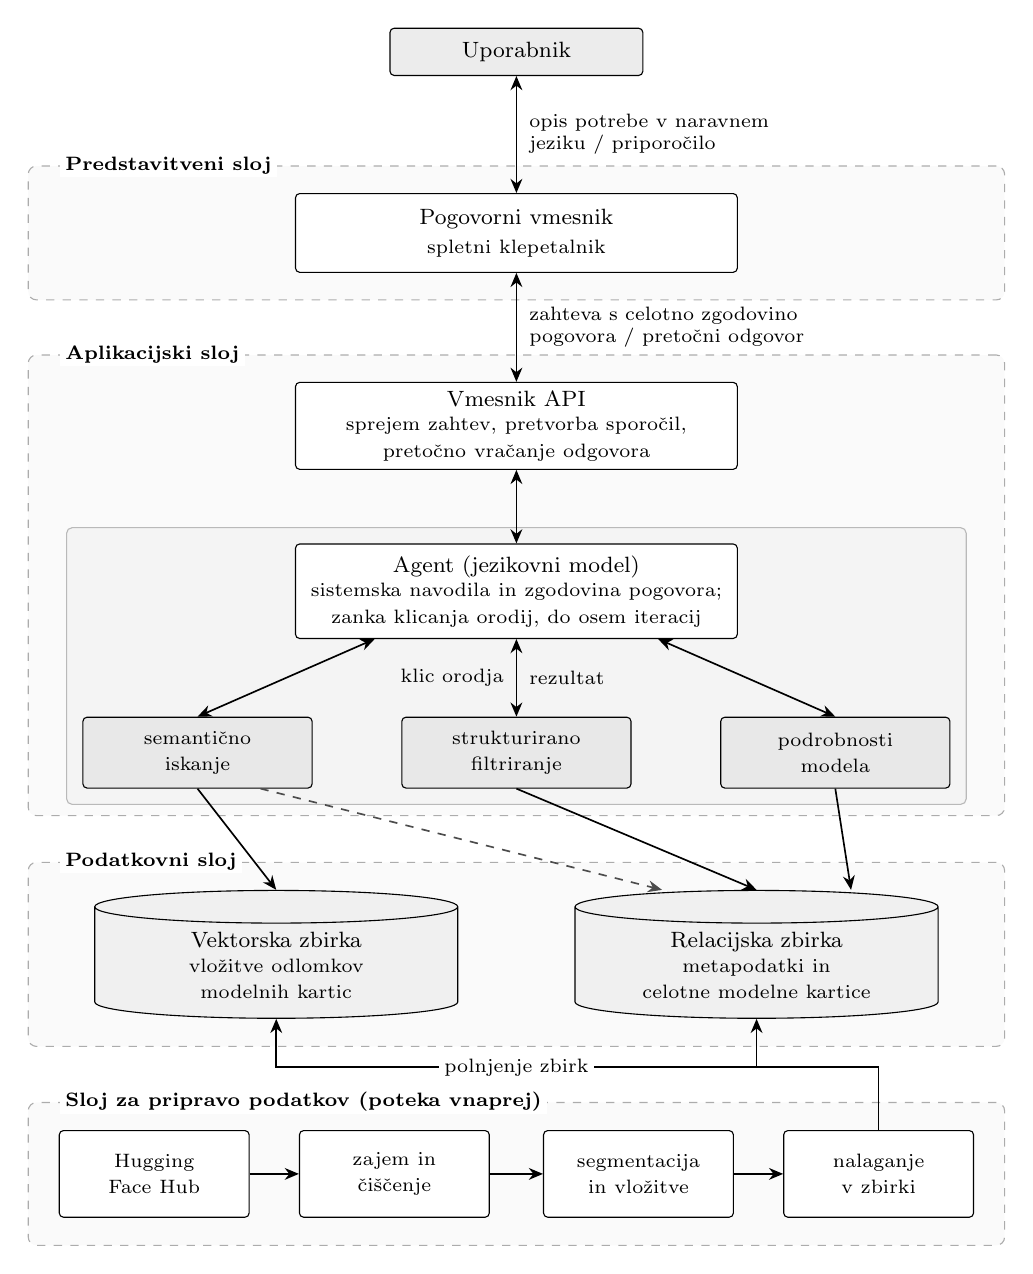
\begin{tikzpicture}[diagram]

% ---------- komponente ----------
\node[blok, fill=gray!15, text width=30mm, minimum height=6mm] (uporabnik) at (0,2.3) {Uporabnik};

\node[blok, text width=54mm, minimum height=10mm] (vmesnik) at (0,0)
    {Pogovorni vmesnik\\[1pt]\scriptsize spletni klepetalnik};

\node[blok, text width=54mm, minimum height=11mm] (api) at (0,-2.45)
    {Vmesnik API\\[1pt]\scriptsize sprejem zahtev, pretvorba sporočil,\\ pretočno vračanje odgovora};

\node[blok, text width=54mm, minimum height=12mm] (agent) at (0,-4.55)
    {Agent (jezikovni model)\\[1pt]\scriptsize sistemska navodila in zgodovina pogovora;\\ zanka klicanja orodij, do osem iteracij};

\node[blok, fill=gray!18, text width=27mm, minimum height=9mm] (o1) at (-4.05,-6.6) {\scriptsize semantično\\ iskanje};
\node[blok, fill=gray!18, text width=27mm, minimum height=9mm] (o2) at (0,-6.6)     {\scriptsize strukturirano\\ filtriranje};
\node[blok, fill=gray!18, text width=27mm, minimum height=9mm] (o3) at (4.05,-6.6)  {\scriptsize podrobnosti\\ modela};

\node[zbirka, text width=44mm, minimum height=16mm] (vek) at (-3.05,-9.3)
    {Vektorska zbirka\\[1pt]\scriptsize vložitve odlomkov\\ modelnih kartic};
\node[zbirka, text width=44mm, minimum height=16mm] (rel) at (3.05,-9.3)
    {Relacijska zbirka\\[1pt]\scriptsize metapodatki in\\ celotne modelne kartice};

\node[blok, text width=22mm, minimum height=11mm] (p1) at (-4.6,-11.95) {\scriptsize Hugging\\ Face Hub};
\node[blok, text width=22mm, minimum height=11mm] (p2) at (-1.55,-11.95) {\scriptsize zajem in\\ čiščenje};
\node[blok, text width=22mm, minimum height=11mm] (p3) at (1.55,-11.95) {\scriptsize segmentacija\\ in vložitve};
\node[blok, text width=22mm, minimum height=11mm] (p4) at (4.6,-11.95) {\scriptsize nalaganje\\ v zbirki};

% ---------- povezave ----------
\draw[tok,<->] (uporabnik) -- node[oznaka, right=1mm, text width=36mm, align=left]
    {opis potrebe v naravnem jeziku / priporočilo} (vmesnik);
\draw[tok,<->] (vmesnik) -- node[oznaka, right=1mm, text width=40mm, align=left]
    {zahteva s celotno zgodovino pogovora / pretočni odgovor} (api);
\draw[tok,<->] (api) -- (agent);

\draw[tok,<->] ([xshift=-18mm]agent.south) -- (o1.north);
\draw[tok,<->] (agent.south) -- node[oznaka, left=1mm] {klic orodja}
                                node[oznaka, right=1mm] {rezultat} (o2.north);
\draw[tok,<->] ([xshift=18mm]agent.south) -- (o3.north);

\draw[tok] (o1.south) -- (vek.north);
\draw[tok, dashed, gray!60!black] ([xshift=8mm]o1.south) -- ([xshift=-12mm]rel.north);
\draw[tok] (o2.south) -- (rel.north);
\draw[tok] (o3.south) -- ([xshift=12mm]rel.north);

\draw[tok] (p1) -- (p2);
\draw[tok] (p2) -- (p3);
\draw[tok] (p3) -- (p4);
\draw[tok] (p4.north) -- ++(0,0.8) -| (vek.south);
\draw[tok] (p4.north) -- ++(0,0.8) -| (rel.south);
\node[oznaka, fill=white, inner xsep=2pt] at (0,-10.6) {polnjenje zbirk};

% ---------- sloji ----------
\begin{scope}[on background layer]
    \node[okvir, fit={(-5.9,0.5) (5.9,-0.5)}] (s1) {};
    \node[okvir, fit={(-5.9,-1.9) (5.9,-7.05)}] (s2) {};
    \node[okvir, fit={(vek) (rel) (-5.9,-9.3) (5.9,-9.3)}] (s3) {};
    \node[okvir, fit={(p1) (p4) (-5.9,-11.95) (5.9,-11.95)}] (s4) {};
    \node[draw=gray!55, rounded corners=2pt, fill=gray!9,
          fit=(agent)(o1)(o3), inner sep=2mm] (jedro) {};
\end{scope}
\node[naslov, anchor=west] at ([xshift=4mm]s1.north west) {Predstavitveni sloj};
\node[naslov, anchor=west] at ([xshift=4mm]s2.north west) {Aplikacijski sloj};
\node[naslov, anchor=west] at ([xshift=4mm]s3.north west) {Podatkovni sloj};
\node[naslov, anchor=west] at ([xshift=4mm]s4.north west) {Sloj za pripravo podatkov (poteka vnaprej)};

\end{tikzpicture}
\end{center}
\caption{Arhitektura sistema AgentPick. Zaledni del obe podatkovni zbirki med
    delovanjem samo bere; polni ju sloj za pripravo podatkov, ki se izvede
    vnaprej in ločeno od obdelave uporabniških zahtev.}
\label{fig:arhitektura}
\end{figure}

Glavno vlogo ima zaledni del, ki koordinira celoten potek obdelave uporabniške zahteve. Po prejemu zahteve izvede analizo uporabnikovega opisa, poišče ustrezne jezikovne modele ter pripravi končni odgovor, ki ga vrne uporabniku. V nadaljevanju so podrobneje opisane vloge posameznih plasti. 

\textbf{Predstavitveni sloj} zajema spletni uporabniški vmesnik v obliki klepetalnika. Uporabnik v naravnem jeziku opiše svoje potrebe, na primer nalogo, omejitve strojne opreme ali želeno velikost modela, vmesnik pa prikazuje generirani odgovor in omogoča nadaljevanje pogovora z dodatnimi vprašanji. 

\textbf{Aplikacijski sloj} predstavlja zaledno storitev, sestavljeno iz dveh delov. Prvi del je vmesnik API, ki skrbi za sprejem zahtev, pretvorbo med zapisi sporočil ter vračanjem odgovorov. Drugi je pa agentni del, velik jezikovni model, ki ob vsaki zahtevi prejme sistemska navodila, zgodovino pogovora in nabor orodij za dostop do kataloga. Orodja so implementirana kot deterministične funkcije nad podatkovnim slojem, zato je mogoče vsak podatek v odgovoru izslediti do konkretne poizvedbe. Pomembna zasnovna odločitev je, da zaledna storitev ne hrani stanja pogovorov: odjemalec ob vsaki zahtevi pošlje celotno zgodovino pogovora, ki agentu služi kot kontekst za razumevanje nadaljnih vprašanj. V nadaljnem razvoju bi ta pristop nadgradili z tako imenovanim drsečim oknom, kjer agent vidi zadnjih nekaj sporočil.

\textbf{Podatkovni sloj} sestavljata dve dopolnjujoči se podatkovni zbirki. Vektorska zbirka hrani vložitve odlomkov modelnih kartic in omogoča semantično iskanje: poizvedbo in odlomke primerja v skupnem vektorskem prostoru, zato najde vsebinsko sorodne modele tudi takrat, kadar se besedišče uporabnikovega opisa ne ujema z besediščem iz dokumentacije. Relacijska zbirka hrani metapodatke o modelih (število prenosov in všečkov, oznake, število parametrov, ...) ter celotne modelne kartice, s čimer omogoča natančno filtriranje, urejanje in odgovarjanje. Delitev na dve zbirki izhaja iz dveh bistveno različnih tipov poizvedb, ki ju mora sistem podpirati: vsebinskega iskanja ter natančnega filtriranja po formalnih kriterijih. 

\textbf{Sloj za pripravo podatkov} deluje ločeno od preostalega sistema in se izvaja v naprej. Obsega pridobivanje metapodatkov in modelnih kartic s portala Hugging Face, njihovo čiščenje in segmentacijo, izračun vložitev ter polnjenje obeh podatkovnih zbirk. Ker je ta obdelava računsko zahtevna in dolgotrajna, je povsem ločena od obdelave uporabniških zahtev: katalog se lahko osvežuje neodvisno, ne da bi to vplivalo na odzivnost sistema, zaledni del pa podatkovni zbirki med delovanjem zgolj bere. 



\section{Potek delovanja agenta}

Ob sprejemu zahteve se modelu poda sistemska navodila, opise treh orodji in celotno zgodovino pogovora. Model se nato v vsakem krogu zanke odloči bodisi pokliče eno ali več orodij bodisi napiše končni odgovor. Rezultati orodij se pripnejo v kontekst in model jih v naslednjem krogu upošteva. Poizvedbo lahko nato zoži, razširi, preveri posameznega kandidata ali zaključi. Potek obdelave se tako prilagaja posamezni zahtevi. Na preprosta vprašanja lahko agent odgovori že po enem klicu orodja, zahtevnejša pa sprožijo daljše zaporedje iskanj in preverjanj. Zanka je omejena na osem iteracij, kar omejuje stroške in odzivni čas. V praksi večina zahtev potrebuje bistveno manj iteracij. Obdelava posamezne zahteve poteka po naslednjih korakih: 

\begin{description}
    \item[Sprejem zahteve.] Vmesnik API prejme uporabnikovo sporočilo skupaj s celotno zgodovino pogovora in iz njiju sestavi vhod za agenta. Vhodu doda sistemska navodila, ki opredeljujejo vlogo agenta, pravila utemeljevanja odgovorov, znane posebnosti kataloga in zahtevano obliko odgovora.

    \item[Interpretacija namena.] Jezikovni model iz uporabnikovega opisa razbere nalogo, omejitve in preference ter jih prevede v formalne kriterije poizvedb. Izrecne omejitve velikosti preslika v razpon dopustnega števila parametrov, omejitve strojne opreme pa v tak razpon pretvori s hevrističnim pravilom o porabi pomnilnika: približno 2 GB na milijardo parametrov pri 16-bitnem zapisu uteži oziroma približno 0,7 GB pri 4-bitni kvantizaciji~\cite{dettmers2023qlora}. Pri tem lahko uporabi lastno znanje za oblikovanje hipotez, na primer o družinah modelov, ki bi ustrezale nalogi, vendar mora vsako hipotezo preveriti v katalogu.

    \item[Pridobivanje kandidatov.] Agent pokliče orodja za poizvedovanje po katalogu. V enem krogu zanke lahko sproži tudi več klicev hkrati. Orodja vrnejo rezultate v strukturirani obliki (JSON), ki se dodajo v kontekst pogovora in so modelu na voljo v naslednjih krogih zanke.

    \item[Iterativno preverjanje.] Model pridobljene rezultate presodi in po potrebi poizveduje znova: sledi referencam v modelnih karticah, na primer na osnovni model ali novejšo različico, ključna dejstva preveri z vpogledom v podrobnosti posameznega modela ter upošteva skupno število zadetkov in opozorila, ki jih vračajo orodja. Sistemska navodila mu izrecno prepovedujejo, da bi dokončen odgovor oprl na eno samo ozko poizvedbo.

    \item[Oblikovanje odgovora.] Ko model presodi, da ima dovolj informacij, najpozneje pa ob dosegu omejitve števila krogov, oblikuje enega od štirih tipov odgovora: (i) rangiran seznam praviloma do treh priporočenih modelov, pri čemer vsakega pospremi kratka obrazložitev; (ii) vprašanje, kadar je zahteva premalo določena. V tem primeru najprej pokrije glavne mogoče interpretacije, pogovor pa usmeri z neposrednim vprašanjem; (iii) izrecno sporočilo, da noben model v katalogu ne izpolnjuje zahtev, namesto prisiljenega priporočila; ali (iv) kratko preusmeritev, kadar sporočilo ni povezano z izbiro jezikovnih modelov.

    \item[Vračanje odgovora.] Končni odgovor se uporabniku prikaže na vmesniku.
\end{description}

Zasnova predvideva tudi napake. Če klic orodja spodleti, se napaka modelu vrne kot strukturirano sporočilo, tako da lahko svoj pristop prilagodi, na primer preoblikuje poizvedbo, namesto da bi se obdelava prekinila. Celoten potek obdelave (meje zahtev, posamezni krogi zanke ter vsi klici orodji z argumenti in trajanjem) se beleži v dnevnik aktivnosti, kar omogoča sledljivost odgovorov in analizo delovanja sistema. 

\section{Iskanje in rangiranje kandidatov}

Agent pridobiva kandidatne modele s tremi orodji, od katerih vsako pokriva drugačno vrsto informacij: semantično iskanje vsebinsko opisane potrebe, strukturirano filtriranje in vpogled v podrobnosti posameznega modela za preverjanje dejstev. Rezultati orodij so oblikovani tako, da agent iz njih dobi dovolj konteksta za presojo brez nepotrebnih dodatnih klicev.

\textbf{Semantično iskanje} je namenjeno poizvedbam, pri katerih uporabnik potrebo opiše vsebinsko, na primer \emph{model za povzemanje pravnih dokumentov}. Poizvedba se z istim vložitvenim modelom, kot je bil uporabljen pri gradnji zbirke, pretvori v vektor, nato pa se na podlagi kosinusne podobnosti~\cite{manning2008introduction} iz vektorske zbirke pridobi večje število najbolj podobnih odlomkov modelnih kartic. Ker lahko več pridobljenih odlomkov pripada isti kartici, se zadetki najprej združijo na ravni modelov; model se pri tem rangira po svojem najboljšem odlomku, saj bi povprečenje podobnosti po vseh odlomkih kaznovalo modele z obsežnimi karticami, pri katerih je relevanten le del vsebine. Tako urejeni kandidati se nato obogatijo z metapodatki iz relacijske zbirke. Sledi ključni korak združevanja različic: katalog namreč vsebuje veliko ponovnih objav istih modelov v drugačnih zapisih (kvantizirane različice GGUF, AWQ, GPTQ ipd.) s skoraj enakimi modelnimi karticami, zato bi brez združevanja seznam rezultatov zapolnile kopije istega modela. Ponovne objave zato združimo v družine, vsako družino pa v rezultatih zastopa en sam predstavnik: praviloma izvirna objava, med več možnostmi pa tista z največjim številom prenosov. Orodje vrne omejeno število najbolje uvrščenih modelov, vsakega opremljenega z metapodatki, morebitno oznako ponovne objave in najrelevantnejšim izsekom kartice.

\textbf{Strukturirano filtriranje} je namenjeno natančnim pogojem in razvrščanju. Kandidate izbira s kombinacijo filtrov po tipu naloge, oznakah, delu identifikatorja in razponu števila parametrov, rezultate pa uredi po izbranem kriteriju: po številu prenosov, številu všečkov, velikosti ali datumu zadnje spremembe. S tem lahko agent zanesljivo odgovarja na vprašanja, kot sta \emph{največji model za pisanje kode} ali \emph{najbolj priljubljen model za prevajanje}, ki jih s semantičnim iskanjem ni mogoče korektno nasloviti. Poleg seznama zadetkov orodje vrne tudi skupno število vseh modelov, ki ustrezajo filtrom, in samodejno ustvarjena opozorila. Ta agenta opozorijo na tri značilne pasti kataloga: na redko uporabljene oznake, pri katerih je verjetneje, da je izbrana oznaka napačna, kot da iskana zmožnost v katalogu ne obstaja (orodje ob tem predlaga podobne obstoječe oznake); na modele, ki so bili iz velikostnega filtra izključeni zgolj zato, ker njihovo število parametrov ni znano; ter na iskanje najmanjših modelov brez dodatnih pogojev, pri katerem spodnji del kataloga zasedajo pomanjšani raziskovalni modeli, neprimerni za dejansko uporabo. Na podlagi teh informacij lahko agent loči primer, ko ustrezni modeli res ne obstajajo, od primera, ko je zgolj filter preozek, in poizvedbo ustrezno preoblikuje.

\textbf{Vpogled v podrobnosti modela} vrne celotne metapodatke in obsežnejši del modelne kartice za en, natančno določen model. Agent ga uporablja za preverjanje dejstev pred končnim priporočilom, na primer dejanske velikosti ali podprtih jezikov, ter za primerjavo ožjega izbora kandidatov.

Vsa orodja iz rezultatov samodejno izločajo testne artefakte, torej naključno inicializirane modele, ki so na portalu objavljeni za potrebe testiranja programskih knjižnic in niso uporabni jezikovni modeli.

Končno razvrščanje je sestavljeno tako, da orodja opravijo deterministično predizbiro in ureditev kandidatov po posameznih kriterijih (podobnost, priljubljenost, velikost), vsebinsko tehtanje med kandidati pa je prepuščeno jezikovnemu modelu, ki edini pozna celoten kontekst pogovora. Pri izboru upošteva ujemanje specializacije modela z uporabnikovo nalogo, skladnost velikosti z omejitvami strojne opreme ter priljubljenost kot kazalnik razširjenosti in podpore skupnosti, ne pa kakovosti. Rezultat je kratek rangiran seznam priporočil, v katerem je vsak predlagani model utemeljen s podatki, pridobljenimi v opisanem procesu.

Celoten opisani potek je izveden v programskem jeziku Python z uporabo ogrodja za razvoj agentov Microsoft Agent Framework; uporabljene tehnologije in podrobnosti izvedbe posameznih komponent predstavljamo v poglavju~\ref{ch:implementacija}.




%----------------------------------------------------------------
% Poglavje (Chapter) 4
%----------------------------------------------------------------
\chapter{Implementacija}
\label{ch:implementacija}

Zasnovo iz prejšnjega poglavja smo uresničili kot odprtokodno spletno aplikacijo. V tem poglavju najprej predstavimo izbrane tehnologije, nato cevovod za zajem in predobdelavo podatkov, zaledno storitev z agentom in orodji ter uporabniški vmesnik. Celoten sistem --- vmesnik, zaledje in obe podatkovni bazi --- se postavi z enim ukazom prek orodja Docker Compose\footnote{\url{https://docs.docker.com/compose/}, dostopano 14.~7.~2026}.

\section{Izbor tehnologij}
\label{sec:tehnologije}

Pregled uporabljenih tehnologij po slojih arhitekture podaja Tabela~\ref{tab:tehnologije}.

\begin{table}[htbp]
\centering
\begin{tabular}{lll}
\hline
\textbf{Sloj} & \textbf{Komponenta} & \textbf{Tehnologija} \\
\hline
predstavitveni & pogovorni vmesnik & Open WebUI \\
aplikacijski & spletna storitev & FastAPI (Python) \\
aplikacijski & agent in orodja & Microsoft Agent Framework \\
aplikacijski & jezikovni model & \texttt{gpt-5.4-mini} \\
podatkovni & semantično iskanje & Qdrant \\
podatkovni & metapodatki in kartice & PostgreSQL 16 \\
priprava podatkov & vložitve & \texttt{BAAI/bge-large-en-v1.5} \\
priprava podatkov & vmesni zapis & Apache Parquet \\
namestitev & orkestracija & Docker Compose \\
\hline
\end{tabular}
\caption{Uporabljene tehnologije po slojih sistema.}
\label{tab:tehnologije}
\end{table}

Zaledni del je napisan v Pythonu z ogrodjem FastAPI\footnote{\url{https://fastapi.tiangolo.com}, dostopano 14.~7.~2026}, ki podpira asinhrono obdelavo zahtev in samodejno generira dokumentacijo programskega vmesnika. Za agentni del uporablja ogrodje Microsoft Agent Framework, ki poskrbi za zanko klicanja funkcij z nastavljivo omejitvijo iteracij, pretvorbo definicij orodij v obliko vmesnika jezikovnega modela ter pretočno vračanje odgovorov; jedra agentne logike nam tako ni bilo treba izumljati na novo, kar zmanjša možnost napak.

Vektorizirani podatki so shranjeni v vektorski bazi Qdrant, strukturirani podatki pa v relacijski bazi PostgreSQL. Qdrant podpira kosinusno podobnost z indeksom HNSW in ob vektorjih hrani poljubne metapodatke, PostgreSQL pa učinkovito izvaja filtriranje, razvrščanje in agregacije, ki jih potrebujejo strukturirane poizvedbe. Vložitve --- tako pri gradnji kataloga kot pri poizvedbah med delovanjem --- računa model \texttt{BAAI/bge-large-en-v1.5} prek knjižnice \texttt{sentence-transformers}\footnote{\url{https://www.sbert.net}, dostopano 14.~7.~2026}, kar pomeni, da semantično iskanje ne potrebuje zunanjih storitev in da sta poizvedba in katalog zagotovljeno v istem vektorskem prostoru.

Za veliki jezikovni model je uporabljen \texttt{gpt-5.4-mini}. Ta ima dosti večjo zmogljivost kot različica nano in je priporočen za agentne sisteme, saj ima večjo sposobnost načrtovanja in uporabe orodij. Za agentni sistem v tej nalogi je to še posebej smiselno, saj ima sistem enega samega agenta, ki je hkrati načrtovalec, ima na voljo tri orodja in po potrebi iterira --- celotno breme odločanja torej nosi en model. Model je nastavljiv prek okoljske spremenljivke, zato je mogoče sistem brez posegov v kodo poganjati tudi z drugimi modeli ali prek združljivih končnih točk.

\section{Zajem in predobdelava podatkov}
\label{sec:podatki}

Podatki o modelih so bili zajeti s portala Hugging Face Hub, ki je eden največjih javnih repozitorijev modelov umetne inteligence. Portal omogoča dostop do modelov, njihovih metapodatkov ter pripadajoče dokumentacije v obliki kartic modelov. Celoten cevovod, od zajema do napolnjenih podatkovnih zbirk, prikazuje Slika~\ref{fig:cevovod}; posamezne korake opisujemo v nadaljevanju.

\begin{figure}[htbp]
\begin{center}
\linespread{1}\selectfont
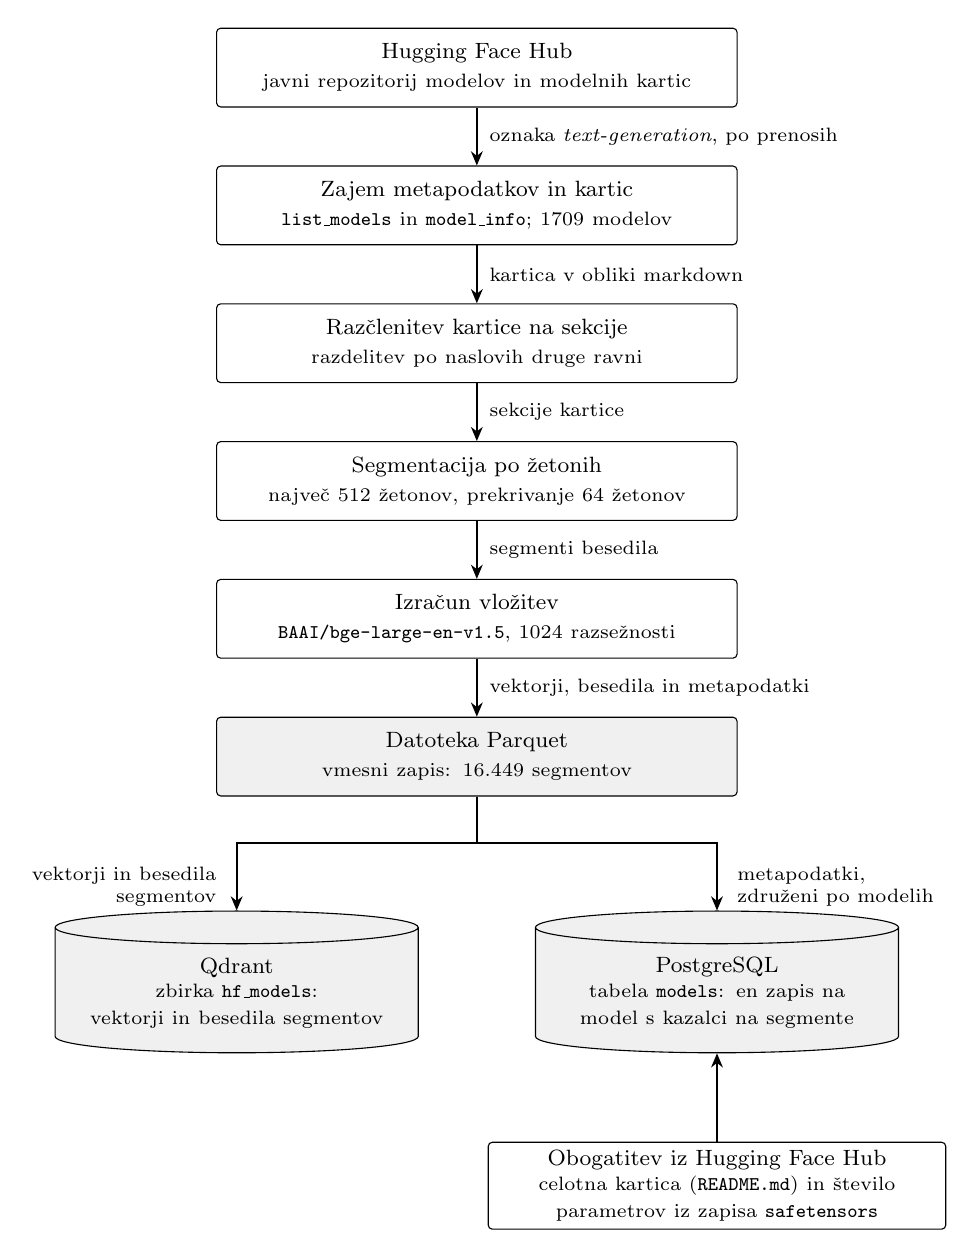
\begin{tikzpicture}[diagram]

\node[blok, text width=64mm, minimum height=10mm] (hf) at (0,0)
    {Hugging Face Hub\\[1pt]\scriptsize javni repozitorij modelov in modelnih kartic};
\node[blok, text width=64mm, minimum height=10mm] (zajem) at (0,-1.75)
    {Zajem metapodatkov in kartic\\[1pt]\scriptsize \texttt{list\_models} in \texttt{model\_info}; 1709 modelov};
\node[blok, text width=64mm, minimum height=10mm] (sekcije) at (0,-3.5)
    {Razčlenitev kartice na sekcije\\[1pt]\scriptsize razdelitev po naslovih druge ravni};
\node[blok, text width=64mm, minimum height=10mm] (segmenti) at (0,-5.25)
    {Segmentacija po žetonih\\[1pt]\scriptsize največ 512 žetonov, prekrivanje 64 žetonov};
\node[blok, text width=64mm, minimum height=10mm] (vlozitve) at (0,-7.0)
    {Izračun vložitev\\[1pt]\scriptsize \texttt{BAAI/bge-large-en-v1.5}, 1024 razsežnosti};
\node[blok, fill=gray!12, text width=64mm, minimum height=10mm] (parquet) at (0,-8.75)
    {Datoteka Parquet\\[1pt]\scriptsize vmesni zapis: 16.449 segmentov};

\coordinate (razcep) at (0,-9.85);

\node[zbirka, text width=44mm, minimum height=18mm] (qdrant) at (-3.05,-11.75)
    {Qdrant\\[1pt]\scriptsize zbirka \texttt{hf\_models}:\\ vektorji in besedila segmentov};
\node[zbirka, text width=44mm, minimum height=18mm] (pg) at (3.05,-11.75)
    {PostgreSQL\\[1pt]\scriptsize tabela \texttt{models}: en zapis na\\ model s kazalci na segmente};

\node[blok, text width=56mm, minimum height=11mm] (obog) at (3.05,-14.2)
    {Obogatitev iz Hugging Face Hub\\[1pt]\scriptsize celotna kartica (\texttt{README.md}) in število\\ parametrov iz zapisa \texttt{safetensors}};

\draw[tok] (hf) -- node[oznaka, right=1mm] {oznaka \emph{text-generation}, po prenosih} (zajem);
\draw[tok] (zajem) -- node[oznaka, right=1mm] {kartica v obliki markdown} (sekcije);
\draw[tok] (sekcije) -- node[oznaka, right=1mm] {sekcije kartice} (segmenti);
\draw[tok] (segmenti) -- node[oznaka, right=1mm] {segmenti besedila} (vlozitve);
\draw[tok] (vlozitve) -- node[oznaka, right=1mm] {vektorji, besedila in metapodatki} (parquet);

\draw[semithick] (parquet.south) -- (razcep);
\draw[tok] (razcep) -| (qdrant);
\draw[tok] (razcep) -| (pg);
\node[oznaka, anchor=east, align=right] at (-3.25,-10.4) {vektorji in besedila\\ segmentov};
\node[oznaka, anchor=west, align=left]  at (3.25,-10.4)  {metapodatki,\\ združeni po modelih};

\draw[tok] (obog) -- (pg);

\end{tikzpicture}
\end{center}
\caption{Cevovod za zajem in predobdelavo podatkov: od zajema s portala
    Hugging Face Hub prek razčlenitve kartic in izračuna vložitev do polnjenja
    obeh podatkovnih zbirk.}
\label{fig:cevovod}
\end{figure}

Zajem je implementiran v programskem jeziku Python z uporabo knjižnice \texttt{huggingface\_hub}\footnote{\url{https://github.com/huggingface/huggingface_hub}, dostopano 14.~7.~2026}. Seznam modelov pridobimo z metodo \texttt{list\_models}, pri čemer filtriramo po oznaki naloge \emph{text-generation} in modele obiskujemo po padajočem številu prenosov. Za izboljšanje kakovosti podatkov je uporabljen prag minimalne popularnosti: v katalog so vključeni modeli z vsaj 1000 prenosi. S tem katalog omejimo na modele z dejansko uporabo, pri katerih sta dokumentacija in vzdrževanje praviloma boljša. Tako zgrajeni posnetek stanja obsega 1709 modelov.

Za vsak model nato z metodo \texttt{model\_info} pridobimo naslednje metapodatke: število prenosov, število všečkov, oznake, oznako naloge (\texttt{pipeline\_tag}), uporabljeno knjižnico, datum nastanka modela ter datum zadnje spremembe.

Poleg metapodatkov pridobimo za vsak model tudi kartico modela v obliki datoteke markdown. Te niso enotne po obliki, zato smo implementirali lasten postopek razčlenjevanja dokumentov. Dokumenti so razdeljeni glede na naslove druge ravni, iz česar nastanejo sekcije, kjer vsaka predstavlja semantično zaokroženo vsebinsko enoto --- na primer opis modela, uporaba, omejitve ali rezultati meritev.

Po razdelitvi na sekcije sledi dodatna razčlenitev besedila na manjše dele. Vložitveni modeli namreč podpirajo omejeno dolžino vhodnega besedila, zato celotnih sekcij pogosto ni mogoče pretvoriti v vložitve brez izgube podatkov. Razčlenitev je izvedena glede na število žetonov (angl. \emph{token-based chunking}) z razčlenjevalnikom istega modela \texttt{BAAI/bge-large-en-v1.5}, tako da meje segmentov ustrezajo dejanskim omejitvam vložitvenega modela. Največja dolžina segmenta je 512 žetonov, prekrivanje med sosednjimi segmenti pa 64 žetonov. Prekrivanje je pomembno za zmanjšanje izgube informacij na mejah segmentov, s čimer se izboljša semantična predstavitev vsebine.

Za generiranje vložitev je uporabljen model \texttt{BAAI/bge-large-en-v1.5}, implementiran prek knjižnice \texttt{sentence-transformers}; vsak segment se preslika v 1024-razsežni vektor. Segmenti se sproti zapisujejo v datoteko Parquet --- vsaka vrstica ustreza enemu segmentu in vsebuje njegov vektor, besedilo, naslov sekcije, zaporedne indekse ter metapodatke modela. Cevovod si obdelane modele beleži v posebno datoteko, zato se lahko prekinjeni zagon nadaljuje, kjer je ostal. Končni katalog obsega 16.449 segmentov; obdelava teče s hitrostjo približno pol modela na sekundo na običajnem procesorju, na grafičnem procesorju pa nekajkrat hitreje.

Datoteka Parquet je vmesni izdelek, ki ga uporabita dva nalagalnika. Prvi vektorje in besedila segmentov naloži v zbirko \texttt{hf\_models} v bazi Qdrant (kosinusna razdalja, razsežnost 1024); identifikator segmenta postane identifikator točke, preostali stolpci pa njen tovor. Drugi nalagalnik pripravi relacijsko bazo: počaka na dostopnost strežnika PostgreSQL, ustvari shemo, vrstice iz datoteke Parquet združi po modelu in za vsak model vstavi ali posodobi en zapis s metapodatki ter seznamom identifikatorjev pripadajočih segmentov, ki zapise povezuje s točkami v vektorski bazi. Ker oba nalagalnika uporabljata operacijo vstavi-ali-posodobi, je njun ponovni zagon varen.

Sledi še obogatitvena faza, ki za vsak model z vmesnika Hugging Face pridobi celotno kartico (surovi \texttt{README.md}) in število parametrov iz zapisa \texttt{safetensors}. Prav ta vir velikosti je vzrok za pomanjkljivosti, opisane v razdelku~\ref{sec:lastnosti-podatkov}: pri modelih brez tega zapisa vrednost manjka (110 modelov), pri kvantiziranih ponovnih objavah pa je lahko podcenjena. Šuma v podatkih pri zajemu namenoma ne čistimo: katalog ostane zvest posnetek stanja platforme, njegovo interpretacijo --- zlaganje ponovnih objav, izločanje artefaktov, opozorila --- pa v celoti izvaja poizvedbena plast, opisana v razdelku~\ref{sec:orodja}. Tako je ločnica med podatki in njihovo interpretacijo jasna, interpretacijo pa je mogoče izboljševati brez ponovnega zajema.

\section{Zaledni del}
\label{sec:zaledje}

Zaledna storitev je organizirana v dve plasti: tanko spletno plast, ki skrbi za protokol, in agentno jedro z orodji ter dostopom do podatkov.

\subsection{Programski vmesnik}

Storitev izpostavlja programski vmesnik, združljiv z vmesnikom OpenAI: končno točko \texttt{POST /v1/chat/completions} za pogovor (z podporo pretočnemu vračanju prek dogodkov strežnika), \texttt{GET /v1/models}, ki odjemalcem predstavi navidezni model \texttt{agentpick-recommender}, in \texttt{GET /health} za preverjanje delovanja. Združljivost s tem de facto standardom (zahteva N2) pomeni, da lahko sistem uporablja katerikoli obstoječi odjemalec brez prilagoditev --- v našem primeru Open WebUI, enako pa tudi ukazna vrstica ali programske knjižnice. Zahteve so validirane s shemami pydantic, sporočila pa se pretvorijo v obliko, ki jo pričakuje agentno ogrodje.

Poseben primer so opravila v ozadju, ki jih vmesnik Open WebUI pošilja istemu vmesniku: generiranje naslova pogovora, oznak in predlogov nadaljevanj. Ta opravila prepoznamo po značilni obliki poziva in nanje odgovorimo z navadnim klicem jezikovnega modela brez orodij, saj zanje agentna zanka in dostop do kataloga nista potrebna; s tem prihranimo čas in stroške ter ohranimo dnevnik agentnih sledi čist.

\subsection{Agentno jedro}

Agent je definiran kot enkratna (angl. \emph{singleton}) instanca: odjemalec OpenAI z omejitvijo zanke klicanja funkcij na osem iteracij, sistemska navodila iz razdelka~\ref{sec:potek} in tri orodja. Vsaka zahteva se izvede znotraj konteksta, ki ji dodeli identifikator in poskrbi za beleženje; vmesna plast (angl. \emph{middleware}) ob vsakem krogu zanke izmeri približno velikost konteksta in trajanje klica jezikovnega modela. Pri pretočnih zahtevah se deli odgovora uporabniku pošiljajo sproti, ko jih model generira.

\subsection{Orodja in dostop do podatkov}

Orodja so tanki asinhroni ovoji nad podatkovno plastjo. Ker so gonilniki podatkovnih baz blokirajoči, se telo vsakega orodja izvede v delovni niti, tako da med čakanjem na bazo strežnik nemoteno streže druge zahteve. Rezultati se vračajo kot JSON; morebitna napaka se ne razširi kot izjema, temveč se modelu vrne kot polje \texttt{error} v rezultatu --- agent tako napako »vidi« in lahko prilagodi strategijo, na primer z drugačno poizvedbo, namesto da bi celotna zahteva propadla. Opisi orodij in njihovih parametrov so skrbno napisana besedila, saj so del poziva in s tem edina dokumentacija, ki jo model o orodjih dobi.

Dostop do PostgreSQL poteka prek vnaprej odprte zaloge povezav, pri čemer je najmanjše število povezav enako največjemu: agent v istem krogu pogosto sproži več orodij hkrati, zato se vse povezave odprejo ob zagonu in ne sredi zahteve. Skupno število zadetkov (\texttt{total\_matches}) se izračuna z okensko funkcijo \texttt{COUNT(*) OVER ()} v istem povpraševanju kot vrnjene vrstice, predlogi podobnih oznak pa z razgnezdenjem polja oznak. Vložitve poizvedb se predpomnijo, tako da se ponovljena poizvedba ne vlaga znova. Osrednjo logiko zlaganja družin iz razdelka~\ref{sec:orodja} ilustrira naslednji izsek: ključ družine dobimo tako, da iz imena repozitorija odstranimo označevalce formata.

\begin{verbatim}
_QUANT_TOKENS = frozenset({
    "gguf", "awq", "gptq", "mlx", "exl2", "bnb", "nf4",
    "fp8", "fp4", "int4", "int8", "w4a16", "w8a8",
    "4bit", "8bit", "quantized", "onnx", "autoround",
    "unsloth",
})

def _family_key(model_id: str) -> str:
    repo = model_id.split("/", 1)[-1].lower()
    tokens = [t for t in _ID_TOKEN_RE.split(repo)
              if t and t not in _QUANT_TOKENS]
    return "-".join(tokens)
\end{verbatim}

\subsection{Zagon, beleženje in nastavitve}

Storitev začne streči takoj, počasne vire pa ogreje v ozadju: vzporedno naloži vložitveni model (z dvema poskusnima izračunoma, ker so prvi izračuni po nalaganju občutno počasnejši), odpre zalogo povezav in odjemalca vektorske baze ter izvede po en celoten prehod skozi obe poizvedbeni poti, saj prva poizvedba v vsaki bazi plača enkratne stroške nalaganja. Prva prava uporabniška zahteva zato ni upočasnjena.

Vsaka zahteva se beleži v dnevnik dejavnosti: začetek in konec z identifikatorjem, imenom odgovarjajočega sistema in številom sporočil; vsak krog zanke z oceno velikosti konteksta in trajanjem; ter vsak klic orodja z argumenti, številom rezultatov in trajanjem. Dnevnik je bil nepogrešljiv pri razvoju, poleg tega pa omogoča analizo dejanskega obnašanja agenta --- koliko orodij uporabi in kako globoko iterira ---, ki jo uporabimo pri evalvaciji v Poglavju~\ref{ch:evalvacija} (zahteva N4).

Vse nastavitve se berejo iz okoljskih spremenljivk: ključ in identifikator jezikovnega modela, omejitev iteracij zanke, naslova in imena zbirk obeh podatkovnih baz ter raven beleženja. Edina obvezna nastavitev je ključ za dostop do jezikovnega modela.

\section{Uporabniški vmesnik}
\label{sec:ui}

Predstavitveni sloj je spletni klepetalnik, zgrajen na odprtokodnem vmesniku Open WebUI\footnote{\url{https://github.com/open-webui/open-webui}, dostopano 14.~7.~2026}. Lastnega vmesnika nismo razvijali: vse, kar predstavitveni sloj potrebuje --- uporabniške račune in prijavo, shranjevanje in iskanje pogovorov, sprotno izpisovanje odgovorov ter prilagojen prikaz na mobilnih napravah ---, Open WebUI že vsebuje, razvojni napor pa smo tako lahko usmerili v agentno jedro. Odločilno je bilo, da zaledna storitev govori programski vmesnik, združljiv z OpenAI (zahteva N2): vmesnika zato ni bilo treba programsko spreminjati, povežemo ga zgolj z nastavitvami.

Vmesnik gradimo kot lastno sliko Docker. Ker jezikovnih modelov ne poganjamo lokalno in ker semantično iskanje teče v zaledju, sliko zgradimo v okrnjeni različici: brez orodja Ollama, brez podpore za grafične procesorje in brez vgrajenih modelov za vložitve in razpoznavo govora, ki jih Open WebUI sicer uporablja za svoje lastne funkcije. Preostale nastavitve podamo z okoljskimi spremenljivkami: naslov ponudnika modelov kaže na našo zaledno storitev, privzeti in edini ponujeni model je navidezni \texttt{agentpick-recommender} iz razdelka~\ref{sec:zaledje}, prvi registrirani uporabnik pa samodejno postane skrbnik.

Začetni zaslon vmesnika prikazuje Slika~\ref{fig:ui}. Poleg vnosnega polja ponuja nabor šestih predlaganih vprašanj, ki jih ob vsakem prikazu razvrsti naključno. Predloge smo nastavili sami, tako da pokrivajo značilne vrste zahtev iz razdelka~\ref{sec:cilji} --- od natančno omejenih (velikostna meja, vrsta naloge) prek presežnikov do premalo določenih --- in uporabniku že ob prvem stiku pokažejo, kakšna vprašanja sistem pričakuje.

\begin{figure}[htbp]
\begin{center}

\includegraphics[width=\textwidth,height=0.75\textheight,keepaspectratio]{figures/UI.png}
\end{center}
\caption{Začetni zaslon vmesnika AgentPick z vnosnim poljem in predlaganimi vprašanji.}
\label{fig:ui}
\end{figure}

Potek uporabe je preprost: uporabnik v pogovor vpiše svojo potrebo, vmesnik pa zaledju ob vsaki zahtevi pošlje celotno zgodovino pogovora, s čimer sta izpolnjeni zahtevi F8 in N3. Odgovor se izpisuje sproti, medtem ko ga model generira, zato uporabnik prve besede vidi, še preden je agentna zanka končana. Slika~\ref{fig:odgovor} prikazuje odgovor na eno od predlaganih vprašanj: sistem vrne rangiran seznam priporočenih modelov, vsakega s kratko utemeljitvijo, zakaj ustreza zahtevi (zahteva F2), identifikatorji modelov pa so dobesedno prevzeti iz rezultatov orodij (zahteva F3).

\begin{figure}[htbp]
\begin{center}

\includegraphics[width=\textwidth,height=0.75\textheight,keepaspectratio]{figures/response.png}
\end{center}
\caption{Odgovor sistema na vprašanje »I need an instruction-tuned coding model under 15B parameters that I can run locally. What do you recommend?«}
\label{fig:odgovor}
\end{figure}

Opravila v ozadju, ki jih vmesnik samodejno sproža --- generiranje naslova pogovora, oznak in predlogov nadaljevanj ---, streže isto zaledje z navadnimi, orodij prostimi klici, kot je opisano v razdelku~\ref{sec:zaledje}.

Celoten sistem se postavi z ukazom \texttt{docker compose up}: zažene se vmesnik, zaledje ter bazi Qdrant in PostgreSQL, vsaka komponenta v svojem vsebniku s trajnim nosilcem podatkov. Nastavitve --- ključ za jezikovni model, njegov identifikator in skrivnost za podpisovanje sej vmesnika --- se podajo v datoteki \texttt{.env}. Podatkovni cevovod iz razdelka~\ref{sec:podatki} se izvede enkrat ob postavitvi in napolni obe bazi. S tem je izpolnjena zahteva N5, sistem pa je pripravljen za uporabo in za evalvacijo, ki jo opisuje naslednje poglavje.






%----------------------------------------------------------------
% Poglavje (Chapter) 5
%----------------------------------------------------------------
\chapter{Evalvacija}
\label{ch:evalvacija}

\section{Testni primeri}
\section{Rezultati}


%----------------------------------------------------------------
% Poglavje (Chapter) 6
%----------------------------------------------------------------
\chapter{Sklepne ugotovitve}
\label{ch:sklep}


% ---------------------------------------------------------------
% Appendix
% ---------------------------------------------------------------
\appendix
%\addcontentsline{toc}{chapter}{Razširjeni povzetek}
\chapter{Title of the appendix 1}

Example of the appendix.

%----------------------------------------------------------------
% SLO: bibliografija
% ENG: bibliography
%----------------------------------------------------------------
\bibliographystyle{elsarticle-num}


\bibliography{bibliography}



\end{document}
